% ============================================================================
% 片G · sub3 同尺并排对照（上＝源位图按源排印宽 86.0mm；下＝TikZ 重绘同宽 86.0mm）
% 编译：xelatex sub3_对照-600dpi.tex → PyMuPDF 600dpi 栅格化 → PNG（sub3_对照-600dpi.png）
% （standalone 类正文禁用 \\ / tabular，故用 minipage + \par 竖向叠放）
% 另附红/蓝叠加图（源=红、重绘=蓝、重合=黑），由 sub3_build.py 生成
% ============================================================================
\documentclass[border=3mm]{standalone}
\usepackage{graphicx}
\usepackage{tikz}
\usepackage{amsmath}
\usepackage{unicode-math}
\setmathfont{texgyretermes-math.otf}
\usepackage{xeCJK}
\setCJKmainfont{SimSun}
\pagestyle{empty}
\begin{document}
\begin{minipage}{88mm}\centering
  {\small 上：源位图 sub3\_B\_4.png（1408$\times$374px，源排印宽 86.0mm）}\par
  \vspace{1.2mm}
  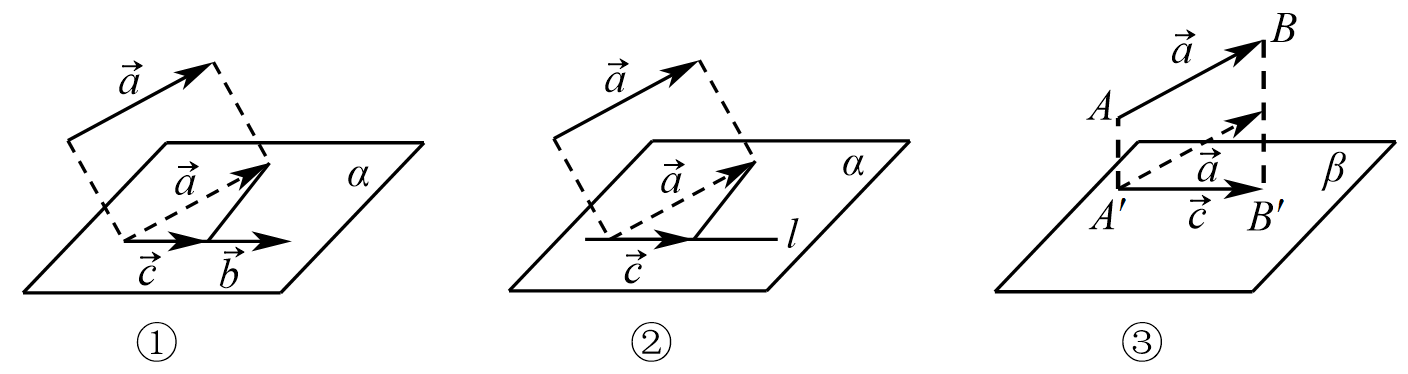
\includegraphics[width=86.0mm]{sub3_source.png}\par
  \vspace{1.0mm}
  {\color[gray]{0.55}\rule{86.0mm}{0.3pt}}\par
  \vspace{1.0mm}
  {\small 下：TikZ 矢量重绘（bbox＝画布 86.0000$\times$22.8440mm，原尺寸置入 86.0mm）}\par
  \vspace{1.2mm}
  % ============================================================================
% 片G · sub3 —— 投影三联图（预习区条目 3 的 ①②③ 三联示意图）TikZ 矢量重绘（逐要素复刻）
% 源位图：工作区/字替对照-0909/variantF/media/media/sub3_B_4.png（1408×374 px）
% 源排印宽 86.0 mm（variantF/sec.tex 原尺寸 3.38583in = 86.0 mm；body.tex 现置入 60 mm）
%
% 【依赖】仅 tikz 本体：不用任何 tikz 库（箭头头部改显式填充多边形，见下端 \head 宏），
%   不引其他宏包。向量标签用 \symbfit（unicode-math 提供）；文件首行已备
%   \providecommand 回落定义，故在纯 tikz（无 unicode-math）环境下同样可编译（字体观感见核对表）。
%
% 【折算基准】1 px = 86.0/1408 = 0.06107955 mm；画布 86.0000 × 22.8440 mm（=1408×374 px）
%   本片段 bbox＝源画布（含四周留白：左 1.34／右 0.73／上 0.79／下 0.73 mm），
%   故整图等比缩放后可与现 \includegraphics 原尺寸互换：
%   body.tex 现置入宽 60 mm ⇒ scale = 60/86.0 = 0.69767
%   （须连字号线宽同缩：用 \resizebox{60mm}{!}{…}；tikz 的 scale= 不缩线宽与字号，勿单用）
%
% 【线宽】源实测灰度质量宽 3.25～4.38 px（中位 3.5 px ＝ 0.2139 mm ≈ 0.607 pt）
%   ⇒ 几何笔画统一取 line width = 0.22 mm；线端 butt（源顶点无出锋）、拐角 miter
%   ⇒ 圈号圆环源实测约 1.6 px（0.10 mm）偏细，单列 line width=0.10 mm
% 【线型】实线：三联平面轮廓各 1 条闭合折线、①② 基线（c 杆+b 杆/l 线，共线实拉通）、
%   ①②自由向量与面内向量、③自由向量 a、③A′B′ 向量；
%   虚线两档（源按 px 实测 → mm）：
%     甲·斜链虚线（①链A/链B/链C、②链A′/链B′/链C′、③中斜向量）：on 14.4px=0.880mm，off 9.0px=0.550mm
%     乙·竖直虚线（③ A–A′、B–B′）：on 18.0px=1.100mm，off 13.3px=0.812mm
%     （A–A′ 首划仅 8 px＝源起笔被截，故加 dash phase=0.611 mm 复现首划长度与相位）
% 【箭头】源头部（P1 b 头灰度剖面实测，10 处头部同制）：长 39 px=2.382 mm、半宽 9.5 px=0.580 mm、
%   背凹口（Stealth 型）凹点距尖端 31.5 px=1.924 mm ⇒ 多边形
%   (0,0)-(-2.382,+0.580)-(-1.924,0)-(-2.382,-0.580)，随箭杆方向旋转。共 10 处：
%   ①自由a、①面内a、①c、①b、②自由a、②面内a、②c、③自由a、③A′B′、③中斜a
% 【字号】源字母实测：A/B 帽高 30 px=1.832 mm ⇒ 字号 1.832/0.662 = 2.768 mm = 7.86 pt
%   （Termes 系帽高 0.662 em；与下行 font= 一致）；β/l 同号；α 源盒仅 20×19px（比同号 x 高略小）
%   ⇒ α 单列 7.11 pt；向量标签 a/c/b 用粗斜体（\symbfit）+ \vec 箭头，字号同；
%   圈号数字高 24 px=1.466 mm ⇒ 6.29 pt（源圈号为 CJK 圈号字，圆环 39px＋数字 24px 分开复刻）
% 【坐标】像素（源图，y 向下）→ TikZ（mm，y 向上）：(x_px, y_px) ↦ (0.06107955·x_px, 0.06107955·(374−y_px))
%   全部顶点由源墨迹最小二乘拟合（平面四边 rms ≤0.25 px；向量杆线 rms ≤0.24 px；虚线端由首末划外推）；
%   重绘↔源逐要素复测（同尺 1:1 栅格）残差 ≤1 px（≤0.06 mm），详见 sub3_逐要素核对表.md
% ============================================================================
\providecommand{\symbfit}[1]{\mathbf{#1}}% 纯 tikz 体检回落（unicode-math 在位时本行不生效）
\def\head#1#2{% #1=尖端坐标  #2=指向角（度，TikZ y 向上）
  \begin{scope}[shift={#1},rotate={#2}]%
    \fill (0,0)--(-2.382,0.580)--(-1.924,0)--(-2.382,-0.580)--cycle;%
  \end{scope}}%
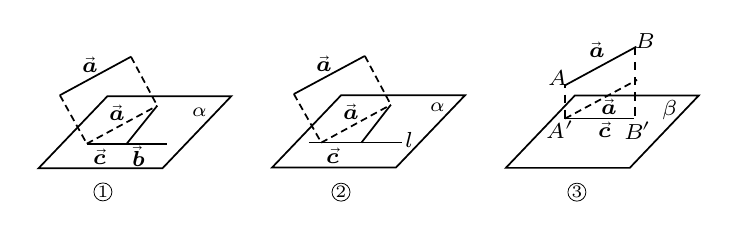
\begin{tikzpicture}[x=1mm,y=1mm,line width=0.22mm,line cap=butt,line join=miter,
                    font=\fontsize{7.86pt}{9.4pt}\selectfont]
  \path[use as bounding box] (0,0) rectangle (86.0000,22.8440);   % bbox＝源画布 1408×374 px

  % ======================= ① 左联 =======================
  % 平面 α：源 px BL(22.44,292.50) BR(280.15,292.50) TR(423.29,142.51) TL(165.76,142.53)
  \draw ( 1.3706, 4.9780) -- (17.1114, 4.9780) -- (25.8544,14.1393) -- (10.1245,14.1381) -- cycle;
  % 虚线链（先画，压在实线之下）：尾-尾、尖-尖、链C（＝向量 a 平移于平面内的虚线拷贝）
  \draw[dash pattern=on 0.880mm off 0.550mm] ( 4.0923,14.2621) -- ( 7.5128, 8.1114); % 链A px(67,140.5)-(123,241.2)
  \draw[dash pattern=on 0.880mm off 0.550mm] (13.1187,19.1539) -- (16.4548,12.9305); % 链B px(214.78,60.41)-(269.4,162.3)
  \draw[dash pattern=on 0.880mm off 0.550mm] ( 7.5128, 8.1114) -- (16.4548,12.9305); % 链C px(123,241.2)-(269.4,162.3)
  % 基线：c 杆 px(123,241.2)→O(206,241.2)；b 杆 O→px(290.5,241.2)（源为一条实拉通线，两处带头）
  \draw ( 7.5128, 8.1114) -- (12.5824, 8.1114);   % c 杆
  \draw (12.5824, 8.1114) -- (17.7436, 8.1114);   % b 杆
  % 面内向量 a：O→px(269.4,162.3)
  \draw (12.5824, 8.1114) -- (16.4548,12.9305);
  % 自由向量 a：px(67,140.5)→(214.78,60.41)（杆线最小二乘拟合 rms 0.2px）
  \draw ( 4.0923,14.2621) -- (13.1187,19.1539);
  % 箭头头部（源 px 尖端）
  \head{(12.5824, 8.1114)}{0}    % c 头，指向 +x（尖端＝O）
  \head{(17.7436, 8.1114)}{0}    % b 头，指向 +x
  \head{(16.4548,12.9305)}{51.22}% 面内 a 头
  \head{(13.1187,19.1539)}{28.46}% 自由 a 头
  % 标签（锚点＝源墨迹盒中心，mm）
  \node[inner sep=0pt] at ( 7.9709,18.1101) {$\vec{\symbfit{a}}$};  % 源盒 px x[119,142] y[61,94]
  \node[inner sep=0pt] at (11.4219,11.9716) {$\vec{\symbfit{a}}$};  % 源盒 px x[175,199] y[161,195]
  \node[inner sep=0pt] at ( 9.1619, 6.4439) {$\vec{\symbfit{c}}$};  % 源盒 px x[139,161] y[252,285]
  \node[inner sep=0pt] at (14.1705, 6.5050) {$\vec{\symbfit{b}}$};  % 源盒 px x[220,244] y[247,288]
  \node[inner sep=0pt,font=\fontsize{7.11pt}{8.5pt}\selectfont] at (21.8665,12.0632) {$\alpha$}; % 源盒 px x[348,368] y[167,186]
  \draw[line width=0.10mm] ( 9.5589, 1.9851) circle[radius=1.1420]; % 圈号① 源圆心 px(156.5,341.5) 外径39px/环宽1.6px
  \node[inner sep=0pt,font=\fontsize{6.29pt}{7.5pt}\selectfont] at (9.5589,1.9851) {1};

  % ======================= ② 中联 =======================
  % 平面 α：源 px BL(508.46,290.50) BR(766.05,290.50) TR(909.45,140.51) TL(651.67,140.57)
  \draw (31.0565, 5.1001) -- (46.7900, 5.1001) -- (55.5488,14.2615) -- (39.8037,14.2578) -- cycle;
  \draw[dash pattern=on 0.880mm off 0.550mm] (33.8075,14.4148) -- (37.2891, 8.2457); % 链A′ px(553.5,138)-(610.5,239)
  \draw[dash pattern=on 0.880mm off 0.550mm] (42.8192,19.2553) -- (46.1212,13.0527); % 链B′ px(701.04,58.75)-(755.1,160.3)
  \draw[dash pattern=on 0.880mm off 0.550mm] (37.2891, 8.2457) -- (46.1212,13.0527); % 链C′ px(610.5,239)-(755.1,160.3)
  % 直线 l（过 O 的水平线，左端 px584.8、右端 px777.5，无箭头）
  \draw (35.7193, 8.2457) -- (47.4893, 8.2457);
  % c 杆：px(610.5,239)→O(694,239)；面内向量 a：O→px(755.1,160.3)；自由 a：px(553.5,138)→(701.04,58.75)
  \draw (37.2891, 8.2457) -- (42.3892, 8.2457);
  \draw (42.3892, 8.2457) -- (46.1212,13.0527);
  \draw (33.8075,14.4148) -- (42.8192,19.2553);
  \head{(42.3892, 8.2457)}{0}    % c 头（尖端＝O）
  \head{(46.1212,13.0527)}{52.18}% 面内 a 头
  \head{(42.8192,19.2553)}{28.24}% 自由 a 头
  \node[inner sep=0pt] at (37.6555,18.2322) {$\vec{\symbfit{a}}$};  % 源盒 px x[605,628] y[59,92]
  \node[inner sep=0pt] at (41.1065,12.0938) {$\vec{\symbfit{a}}$};  % 源盒 px x[661,685] y[159,193]
  \node[inner sep=0pt] at (38.8161, 6.5661) {$\vec{\symbfit{c}}$};  % 源盒 px x[625,646] y[250,283]
  \node[inner sep=0pt,font=\fontsize{7.11pt}{8.5pt}\selectfont] at (52.1009,12.7351) {$\alpha$}; % 源盒 px x[843,863] y[156,175]
  \node[inner sep=0pt] at (48.4361, 8.6122) {$l$};                  % 源盒 px x[788,798] y[218,248]
  \draw[line width=0.10mm] (39.7933, 1.9545) circle[radius=1.1420]; % 圈号② 源圆心 px(651.5,342) 外径39px/环宽1.6px
  \node[inner sep=0pt,font=\fontsize{6.29pt}{7.5pt}\selectfont] at (39.7933,1.9545) {2};

  % ======================= ③ 右联 =======================
  % 平面 β：源 px BL(994.26,291.50) BR(1251.90,291.50) TR(1395.43,141.03) TL(1137.80,141.02)
  \draw (60.7289, 5.0391) -- (76.4655, 5.0391) -- (85.2322,14.2297) -- (69.4963,14.2303) -- cycle;
  % 竖直虚线 A–A′、B–B′（第二档虚线）
  \draw[dash pattern=on 1.100mm off 0.812mm, dash phase=0.611mm] (68.2747,15.6364) -- (68.2747,11.2692); % A–A′ px(1117.8,118)-(1117.8,189.5)
  \draw[dash pattern=on 1.100mm off 0.812mm] (77.1435,20.4250) -- (77.1435,11.2997); % B–B′ px(1263,39.6)-(1263,189)
  % 中斜虚线向量 a′（自 A′ 起、与 a 同向的虚线拷贝，端头带箭头）
  \draw[dash pattern=on 0.880mm off 0.550mm] (68.2564,11.2997) -- (77.3934,16.2166); % px(1117.5,189)-(1267.1,108.5)
  % A′B′ 水平向量：px(1115.5,188.7)→(1261.2,188.7)
  \draw (68.1342,11.3180) -- (77.0335,11.3180);
  % 自由向量 a：A(1118,119.5) → B(1265.6,39.6)
  \draw (68.2869,15.5447) -- (77.3023,20.4250);
  \head{(77.0335,11.3180)}{0}    % A′B′ 头（尖端＝B′）
  \head{(77.3023,20.4250)}{28.43}% 自由 a 头（尖端＝B）
  \head{(77.3934,16.2166)}{28.28}% 中斜 a′ 头
  \node[inner sep=0pt] at (67.2794,16.4304) {$A$};                  % 源盒 px x[1087,1111] y[90,120]
  \node[inner sep=0pt] at (78.3651,21.1641) {$B$};                  % 源盒 px x[1270,1296] y[13,42]
  \node[inner sep=0pt] at (67.6456, 9.8643) {$A'$};                 % 源盒 px x[1089,1126] y[198,229]
  \node[inner sep=0pt] at (77.4797, 9.7422) {$B'$};                 % 源盒 px x[1248,1284] y[199,230]
  \node[inner sep=0pt] at (72.2876,20.0036) {$\vec{\symbfit{a}}$};  % 源盒 px x[1172,1195] y[30,63]
  \node[inner sep=0pt] at (73.8757,12.7656) {$\vec{\symbfit{a}}$};  % 源盒 px x[1198,1221] y[148,182]
  \node[inner sep=0pt] at (73.2955, 9.8949) {$\vec{\symbfit{c}}$};  % 源盒 px x[1189,1211] y[195,229]
  \node[inner sep=0pt] at (81.4801,12.3686) {$\beta$};              % 源盒 px x[1322,1346] y[152,191]
  \draw[line width=0.10mm] (69.7528, 1.9545) circle[radius=1.1420]; % 圈号③ 源圆心 px(1142,342) 外径39px/环宽1.6px
  \node[inner sep=0pt,font=\fontsize{6.29pt}{7.5pt}\selectfont] at (69.7528,1.9545) {3};
\end{tikzpicture}%
% 注：末行 % 必需——\input 时尾随换行会成空格 token，被 standalone/preview 计入裁切框。
\par
\end{minipage}
\end{document}
